\chapter{Design and Implementation of the Proof-of-Concept Application}

Whereas the previous chapters were dedicated in providing a comprehensive literature
review on the topic, we will now focus on the practical implementations of integrating
solutions based on CRDTs in distributed software. In order to achieve this, we will
analyze a use case in which the implementation of CRDT-based data structures proves to be
\textit{valuable}, and document the development of a Proof-of-Concept application built
around that use case.
% TODO: replace the word valuable with something different 

\section{Defining the Use Case for the Proof-of-Concept}

The traditional infrastructure surrounding the broad family of collaborative applications
-- e.g., Google Docs, OneDrive, and many more -- have constantly relied on centralized
coordination paradigms, such as OT. While the approach of designating a central
coordinator for conflict resolution offers distinct advantages -- primarily revolving
around enabling near real-time, non-blocking collaboration and preserving the user's
intention -- there are some contexts in which centralization may present significant
drawbacks, mostly in terms of partition tolerance. For instance, the central coordinator
may be put in a position to be the single point of failure; if it is unreachable, there
is no other node that can approve or order changes, and the operativity of the entire
system collapses\footnote{Some countermeasures can be adopted, such as implementing a
leader election mechanism for designating a new central coordinator node among the nodes
of the network. Nevertheless, this approach would introduce a further layer of complexity
in the distributed system, and would require appropriate handling to enforce
convergence.}.

This precisely illustrates the fundamental advantage of decentralized, peer-to-peer (P2P)
architectures based on CRDTs; through replication across multiple nodes, information is
maintained with high availability and consistency -- i.e., compliant with SEC
constraints. Furthermore, if one or more nodes of the system fail, the system's
operativity is still guaranteed, as updates travel to all active nodes -- whereas the
faulty nodes will reconcile with the system's consistent state, once they come back
online. This approach eliminates the threat of a single point of failure that would
compromise system-wide reliability.

To illustrate this principle, we present a proof-of-concept implementation in the form of
a replicated file storage system that leverages CRDTs to achieve eventual consistency
without the need of centralized conflict resolution mechanisms. This system enables
multiple users to execute fundamental file operations -- including file sharing and
deletion -- on a shared storage infrastructure. 

Furthermore, the solution provides a \textit{file signature} mechanism, through which an
unique user provides a secure method of certifying its ownership over the same file, and
on-demand validity check over the signature can be requested by any other user.

In the following sections, we will refer to the proof-of-concept by the name of
\textit{CRDTSign}. 

\subsection{Proof-of-Concept Scope and Boundaries}

The primary objective that CRDTSign seeks to carry out in its current form is to
serve as a tangible illustration of the capabilities of CRDTs in contemporary
distributed peer-to-peer (P2P) systems. As such, several high-level requirements
must be satisfied:

\begin{itemize}
	\item consistent with the principles of decentralized applications, the backend
		logic is not centralized on a single node, but is served independently at each
		participating node;
	\item because CRDTSign aims to provide an example of modern collaborative software,
		convergence among nodes must be achieved in near real-time -- to satisfy end-user
		expectations for system responsiveness.
\end{itemize}

Conversely, given that the digital signature mechanism is integral to the solution --
serving as a certificate of ownership for files shared by users -- the system must adopt
a cryptographic signature scheme that ensures:

\begin{itemize}
	\item \textit{Integrity}: signatures cannot be altered without detection;
	\item \textit{Authenticity}: the signer's identity can be verified;
	\item \textit{Non-repudiation}: the signer cannot deny having signed the data.
\end{itemize}

As an additional requirement, the system adopts a data retention policy, which ensures
that files whose creation timestamp exceeds a configurable interval -- e.g., 90 days --
are automatically removed from the shared storage. This is made possible to prevent cases
in which the storage's memory becomes saturated over time by files which are unused or
obsolete.

It is worth underlining that the solution developed through CRDTSign poses itself as a
"toy" implementation. While it satisfies the core requirements illustrated above, certain
architectural constraints hinder its expectations of performance in production-grade
environments. For instance, the P2P architecture was not constructed from the ground up;
instead, it was abstracted through the use of a relay server. Rather than enabling direct
node-to-node communication, all messages are routed through the relay server, which in
turn broadcasts them to all peers -- thereby simulating a P2P environment. This design
choice does not fundamentally compromise the decentralized nature of the system, as
concurrency management logic remains managed across individual nodes, rather than being
centralized within the relay server. Additionally, the CRDT data structure was sourced
from an open-source library, and was not custom-made for this application. As we will
discuss in the next chapter, a more robust and scalable solution could be achieved by
designing a domain-specific CRDT structure and message exchange protocol tailored to the
characteristics of the shared data.

\subsection{User Stories}

We will now discuss several use cases of CRDTSign by describing the functionalities of
the system that are available to the end-user.

\paragraph{Uploading a file to storage}
Suppose that \textit{User A} has the need to share a file with a group of users -- e.g.,
\textit{User B} and \textit{User C}. To do so, it possesses a dedicated terminal
(\textit{Node A}), through which it can access CRDTSign's \textit{Web interface}. Once
connected and authenticated in the Web interface, User A uploads the file that it wants
to share to the storage; at this point, the system reads the file, and computes a digital
signature that uniquely identifies User A as the author of the uploaded file. Internally,
the system first adds the file to its local storage, saving its metadata accordingly, and
encapsulates the corresponding change to its state in an update message that is then
broadcast to all other active nodes. Conversely, both Nodes B and C receive the update, 
and autonomously apply it to their respective local storages. After the update is
successfully applied, both User B and User C can visualize the uploaded file and its
metadata in their respective Web interfaces, and can inspect it for further details.

\begin{figure}[tb!]
    \centering
    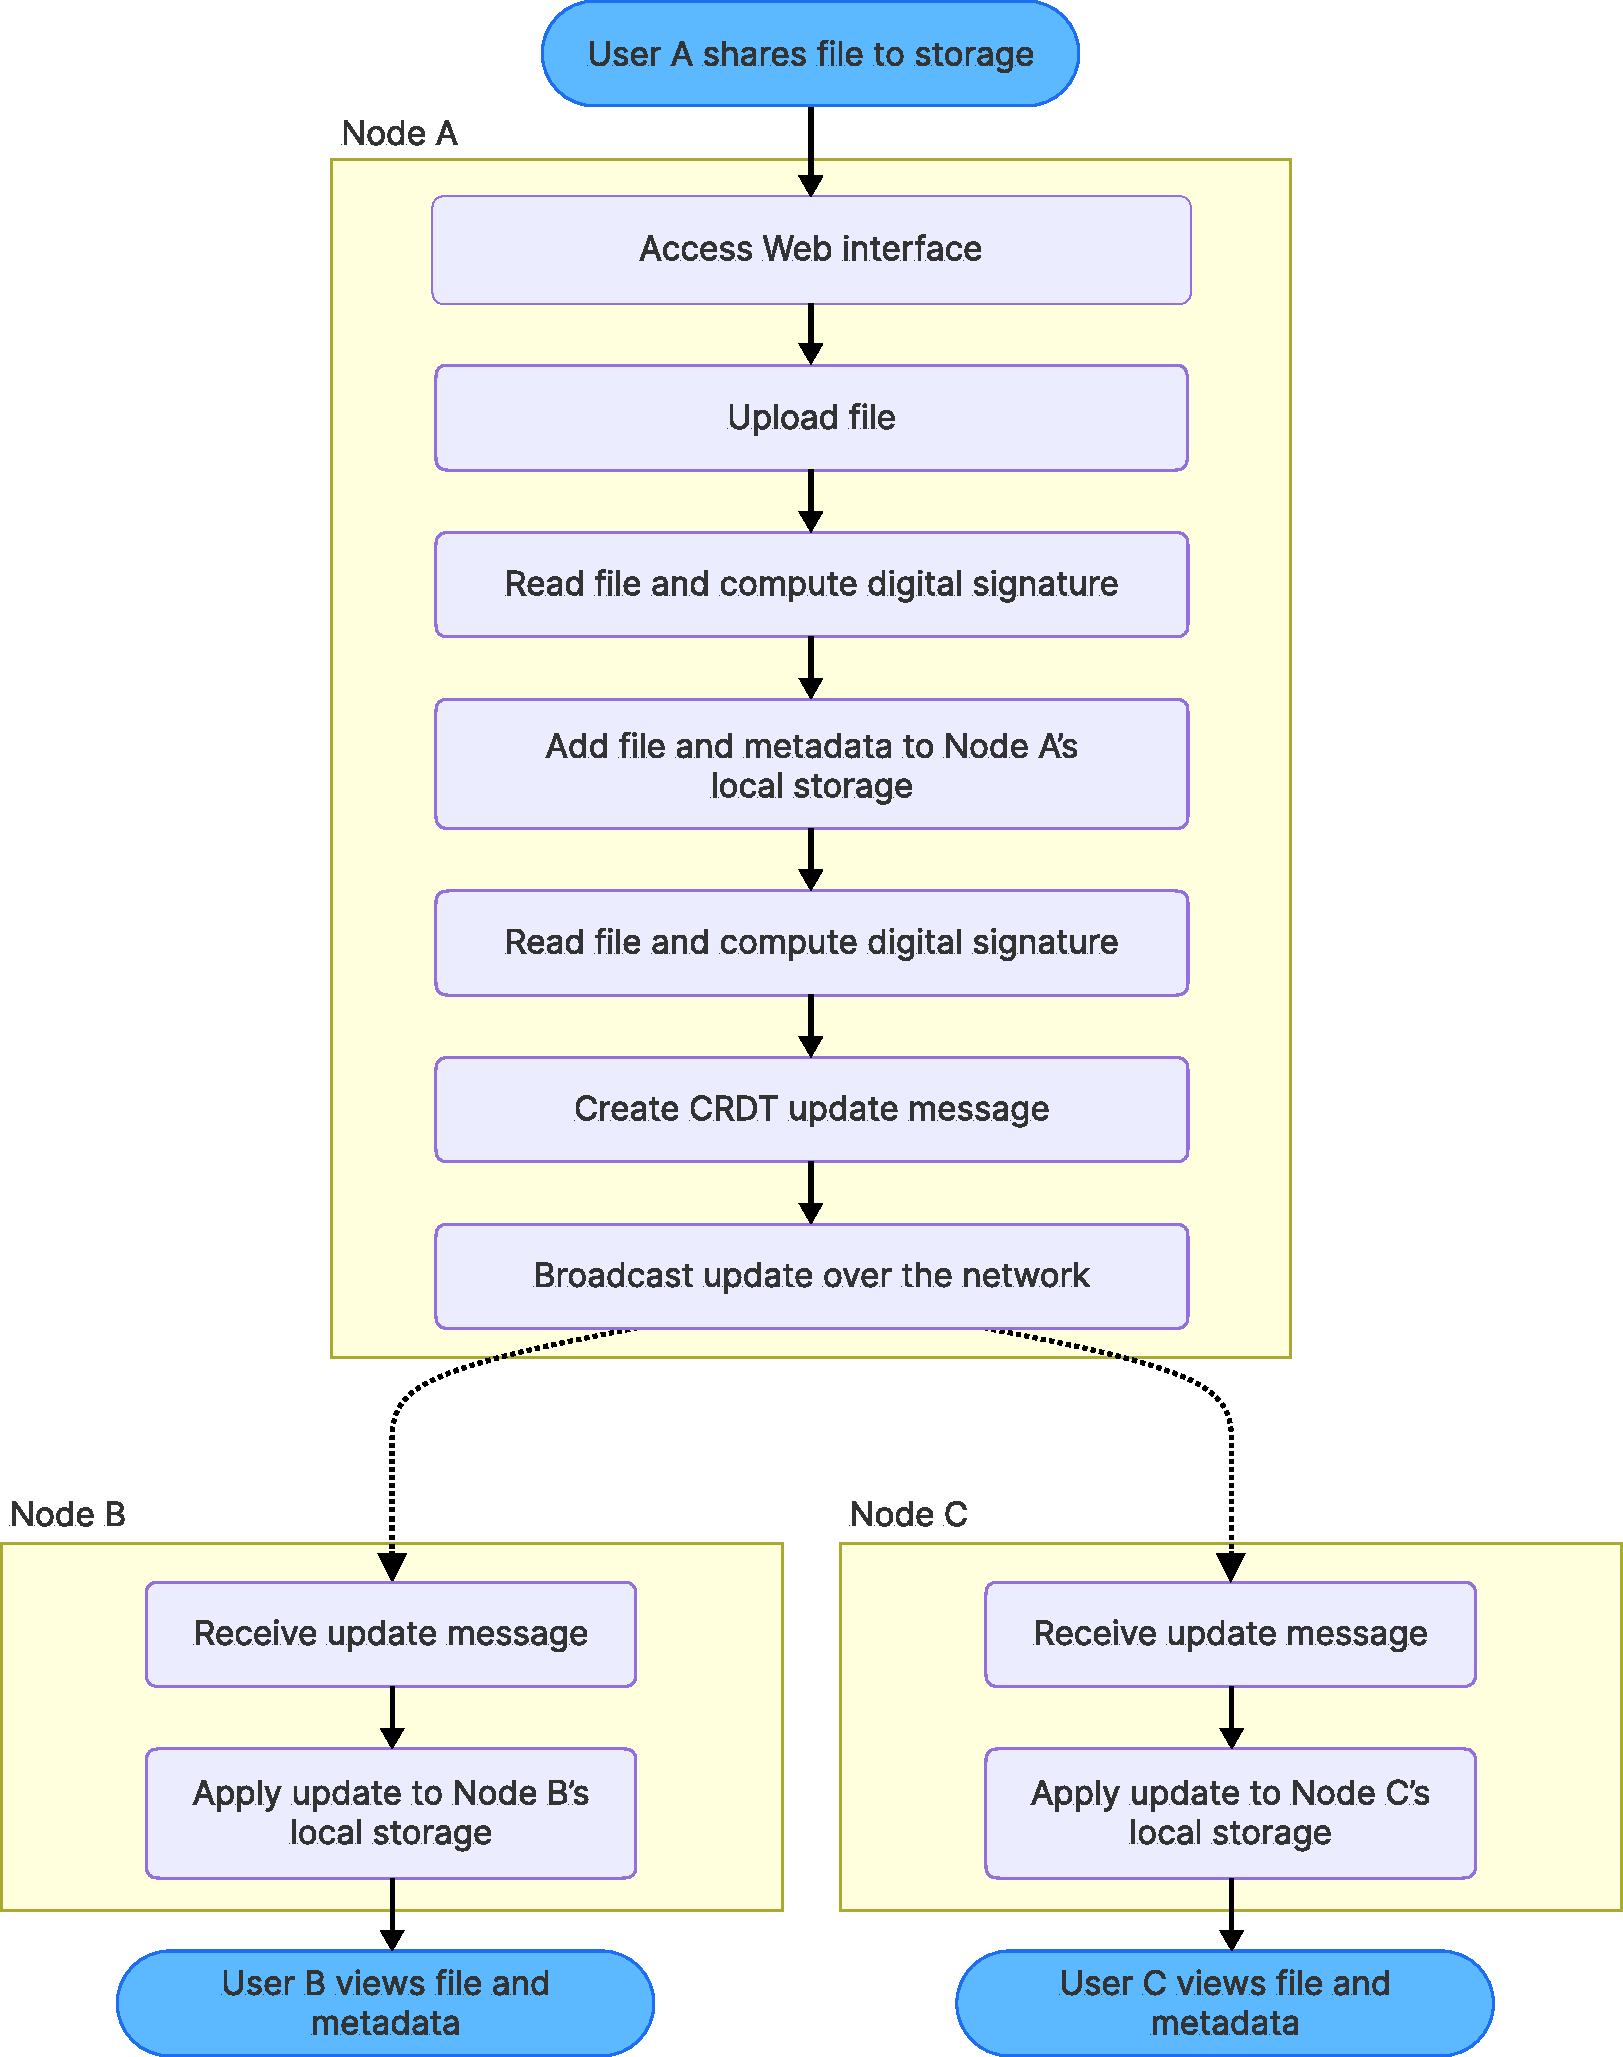
\includegraphics[width=0.8\linewidth]{diagram-file-upload.pdf}
    \caption{High-level flow diagram for the file upload procedure}
    \label{fig:diagram-file-upload}
\end{figure}

\paragraph{Verifying the validity of a file signature}
Suppose now that, once User B receives the file uploaded from User A, it wants to confirm
that the file was indeed uploaded by User A itself. To do so, it can request a
\textit{signature validity check} for the aforementioned file. Consequently, Node B
retrieves the file metadata, combines it with details concerning User A's identity --
i.e., User A's unique identifier -- and uses them to cryptographically validate the
signature to verify. Node B can either assert that the signature is valid, if the
check is successfull, or it is not valid, if the cryptographic validity check fails
with the given parameters. Finally, Node B informs the user -- through a notification
in the Web interface -- of the result of the signature validity check.

\begin{figure}[tb!]
    \centering
    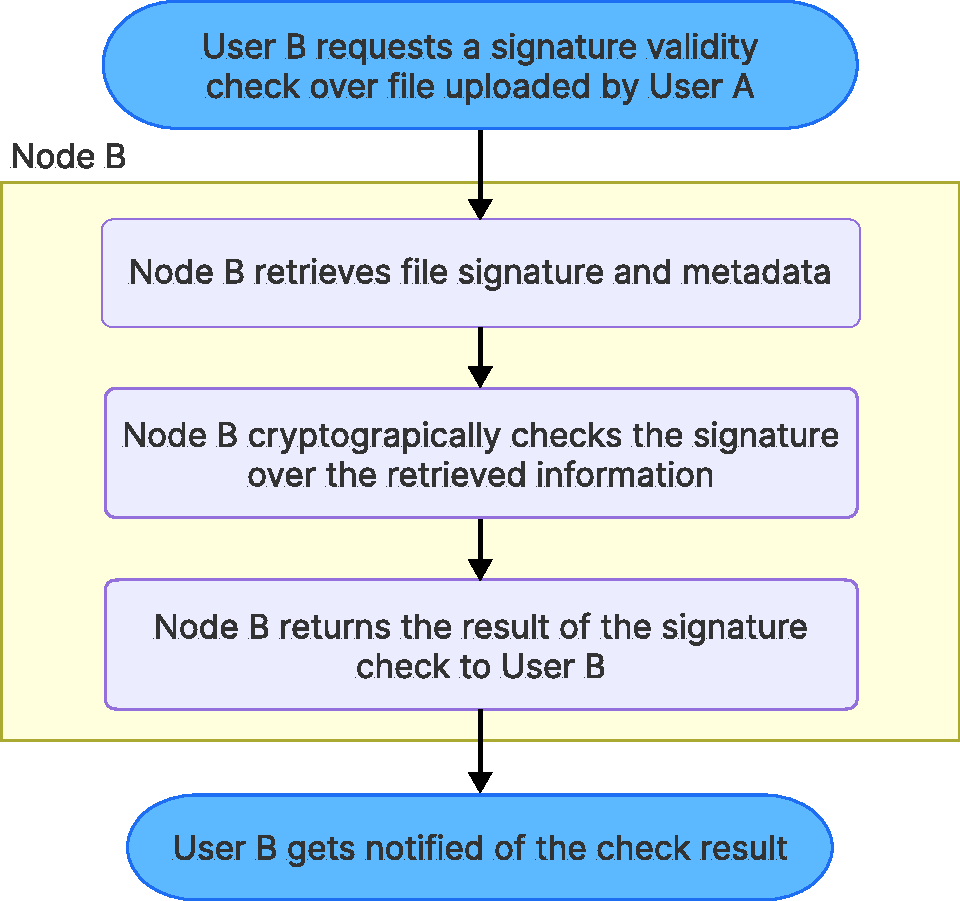
\includegraphics[width=0.61\linewidth]{diagram-signature-check.pdf}
    \caption{High-level flow diagram for the signature check procedure}
    \label{fig:diagram-signature-check}
\end{figure}

\paragraph{Deleting a file from storage}
Having received the file, User C seeks to remove it from storage\footnote{For the sake of
demonstration, whether User C decides to delete the file in agreement with other peers,
or of its own accord -- potentially exposing a malicious intent -- is irrelevant. In a
production-grade application, this can be easily addressed by implementing a
permission-based mechanism, which limits the set of actions a certain user can perform on
files uploaded by other users.}. It can do so by accessing the Web interface, selecting
the file in question, and request its removal from storage. The system responds by first
removing the file from local storage, and then computing an update message that reflects
the node's local state after the file removal. This update is then broadcast to all other
active nodes, which individually apply it to their respective local states -- leading to
a consistent state where the file is removed from storage. The procedure carries out
similarly to what occurs in \autoref{fig:diagram-file-upload}.

\section{System Architecture}

CRDTSign is made up of various components, each carrying out a specific task to achieve
the functionalities that were previously discussed. In the overall distribute network, we
can distinguish between two kinds of node:

\begin{itemize}
	\item \textit{Regular node}: is in charge of accepting and handling the user
		requests, employing both front-end and back-end logic. It is implemented through
		an application written in the
		\textit{Python}\footnote{\url{https://www.python.org/}} programming language,
		which exposes a Web interface through which all of CRDTSign's core
		functionalities are provided to the end-user. When triggered, each functionality
		invokes a custom-made Python library which implements and executes the back-end
		logic locally, interacting with suitable CRDT data structures when required.
		These structures are implemented through
		\textit{pycrdt}\footnote{\url{https://y-crdt.github.io/pycrdt/}}, a library that
		provides bindings to an open-source port of Yjs in the
		\textit{Rust}\footnote{\url{https://rust-lang.org/}} programming language.
	\item \textit{Relay node}: the server in charge of broadcasting messages to regular
		nodes. When a regular node sends an update to the relay node, the latter sends
		the corresponding message to all other nodes that need to receive it.
		Communication between regular nodes and the relay node occurs through the
		\textit{WebSocket} \cite{websocket_rfc} protocol.
\end{itemize}

\begin{figure}[h]
    \centering
    \includegraphics[width=0.61\linewidth]{diagram-system-architecture.pdf}
    \caption{Example of peer-to-peer communication through the relay node -- Node A
		delivers an update to the relay node, and the relay node delivers it to all other
		nodes}
    \label{fig:diagram-system-architecture}
\end{figure}

\section{Software Components}

What follows is a detailed overview concering the design choices that were made over
CRDTSign's code. The code is broadly subdivided into three fundamental blocks; the
back-end, the front-end -- both implemented at the individual, regular node -- and the
relay server.

\subsection{Back-end}

As discussed above, the back-end logic is encapsulated through a custom-made library
that supports all core functionalities of the solution. Namely, CRDTSign's back-end
achieves the following.

Upon bootup, the back-end performs the following checks:

\subsection{Front-end}

\subsection{Relay Server}

\section{Production Deployment}

\section{Development of the Complementary Mobile Application}
